% !TEX root = main.tex

\section{网络层}
\subsection{IP数据报}
\subsubsection{数据传输技术}
\begin{itemize}
\item 电路交换(circuit switching):实际接通一条物理线路,时分多路复用,电话;频分多路复用,电视;一直占用,不管有无数据交互
\item 包交换/分组交换(packet switching):统计多路复用,按需分配;可能引起网络拥塞,适合发送突发数据
\begin{itemize}
	\item 虚电路:需建立连接才可以传输数据(仿照电话系统,因特网之前),好处在于保留带宽
	\begin{itemize}
	    \item 交换式(要交换才建立连接):建立虚电路(VC)表,虚电路标识符(VCI),类似于电话
	    \item 永久式(建立后一直保持):由管理员维护
	\end{itemize}
	\item 数据报(datagram):不需建立连接,因特网,\textbf{不预留带宽}
\end{itemize}
\end{itemize}

IP协议是因特网的网络层协议
\begin{itemize}
\item 可路由的(routable):全局地址,按层分配
\item 尽力服务(best effort):无连接无确认的数据报服务
\item IP协议可以运行在\textbf{任何}网络上,不仅仅是因特网
\end{itemize}

\subsubsection{IP数据报格式}
\begin{itemize}
\item 4个字节一个字,头部最多$(2^4-1)*4=60$B,除选项20B,IPv4选项最多40B,太少了
\item 生存期(TTL)限制在因特网上的停留时间,实际限制为经过的路由器数目,即跳数(hop count),超过则自动清除,防止兜圈,每次经过路由器减1\\
TTL初值默认设置为网络直径的两倍,Windows默认64\\
长了就有捷径(cut-through),因此发展到现在因特网的直径依然在32左右
\item IP数据报一定要封装成帧,通过物理层传输,每次都要修改源和目的地址
\item IP数据报服务类型(type of quality, ToQ),但路由器都没有实现
\end{itemize}

IP数据报的分段和重组
\begin{itemize}
\item 一个物理网络的最大传输单元(maximum transmission unit, MTU)是该网络可以运载的最大有效载荷,即数据帧的数据部分的最大长度\\
如:以太网(DIXv2)的MTU为1500, FDDI和令牌环的MTU分别为4353和4482
\item 只要发出去一定会封装成帧(注意要加头部),帧最长就是MTU,因而要分成多段再分
\item 如果一个数据报的大小大于要承载它的网络的MTU,路由器需要先对该数据报进行分段(fragment)
\item 源主机每次发送IP数据报时都会把标识(Identification)字段加1。
\item 分段时用标识的值保持不变,并且用偏移量字段(offset)指出该片段的数据部分相对原来数据报的偏移量(以8字节为单位),给出原来片段的次序
\item MF(More Fragment), DF(Don't Fragment)
\item 小于MTU-20B,边界,一定要能被8整除,尽可能大(8字节,一定要除掉)
\item IPv6中间不能分段
\item 1400B=512B+512B+376B
\item Path MTU discovery:找到路径上最小的MTU,发现路径上最小MTU
\item 选项最后一定对齐到边界
\item 生存期和头部校验(检验和)会变,其他不变
\end{itemize}

\subsection{IP地址}
48位的MAC地址和32位的IP地址都是全局的(全球分配),但是IP地址空间分层,是可路由的

IP地址可划分为两个部分:
\begin{itemize}
	\item 网络号/网络前缀/网络标识:确定拥有该IP地址的主机位于哪个网络
	\item 主机号:确定属于该网络的哪台主机
\end{itemize}

有类网:ABC单播,D多播,E保留,地址范围如下(点分十进制)
\begin{itemize}
	\item 0 $\thicksim$ 127
	\item 128 $\thicksim$ 191
	\item 192 $\thicksim$ 223
	\item 224 $\thicksim$ 239
	\item 240 $\thicksim$ 255
\end{itemize}

解决IPv4地址不够用的问题
\begin{itemize}
	\item 将一个有类网可以划分为多个相同大小的子网(subnet)\\
用子网掩码(subnet mask)划分边界:主机号全0,剩下的部分(网络号和子网号)全是1\\
子网掩码与IP地址\textbf{相与},若相等则在同个子网中
	\item 变长子网掩码(Variable-length subnet mask, VLSM):允许把一个有类网划分为多个不同大小的子网,类似变长指令集\\
解决主机数目不均匀的问题,如100、50、25、10,则不能等距划分子网\\
用长度来表示子网掩码,如/26代表255.255.255.192
	\item 无类域间路由选择协议(classless inter-domain routing, CIDR):将多个有类网合并为一个更大的网络,称为超网(supernet)\\
可以显著减少路由表中路由的数量,称为路由聚合(route aggregation)
	\item 网络地址转换(network address translation, NAT):将内部地址映射为外部地址的技术(可以扩展6w多倍),将私有地址映射为全局地址\\
NAT将内部源地址转换为外部地址\\
NAPT将端口号也加入NAT的映射中
\end{itemize}

地址解析协议(address resolution protocol, ARP)可以\underline{将IP地址映射为MAC地址}\footnote{也有将也有MAC映射为IP地址的协议}
\begin{itemize}
	\item ARP请求广播帧(谁的IP地址是XXX),ARP响应单播帧(返回MAC地址),IP地址与MAC地址的端口号相同
	\item 没有超时重传机制,超时没有收到响应则丢弃引发ARP查询的IP分组
	\item 源主机获得的映射结果缓存在ARP表中$\lrang{\text{IP address},\text{MAC address},\text{TTL}}$,TTL一般为2到20分钟
	\item 当收到ARP请求,目的主机会缓存源主机的映射,其他主机如果已缓存该映射,则会重置TTL
	\item 也可直接将映射加入ARP缓存,称为静态ARP映射,不会因超时而删除
	\item 源硬件地址和协议地址、目标协议地址都知道,但\textbf{目的硬件地址}不知
\end{itemize}
\begin{figure}[H]
	\centering
	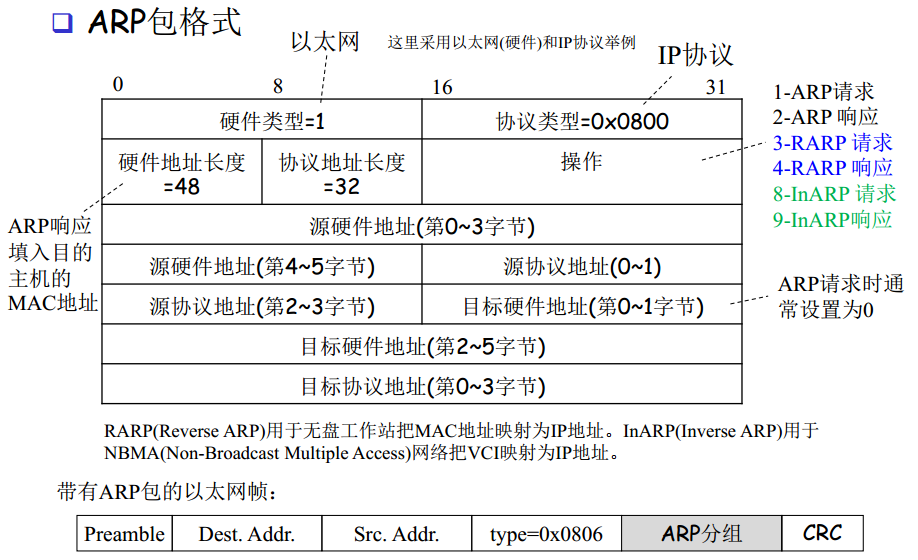
\includegraphics[width=0.7\linewidth]{fig/ARP.PNG}
\end{figure}

DHCP协议(Dynamic Host Configuration Protocol)用于主机在加入网络时\textbf{动态租用}IP地址,用UDP,四个步骤如下
\begin{itemize}
	\item DHCP发现(discover)
	\item DHCP提供(offer)
	\item DHCP请求(request)
	\item DHCP确认(ACK)
\end{itemize}

因特网控制消息协议(Internet Control Message Protocol, ICMP)用于主机或路由器发布网络级别的控制消息,主要是出错/丢包后将信息发回给源主机(TTL减到0、不可达),如回响请求和答复消息(ping)、不可达消息、时间超时消息(原IP头部+原IP数据部份的头64B)、重定位消息

\subsection{路由协议}
有类网的路由选择算法:
利用数据包中的\textbf{目的地址}得到\textbf{目的网络号},然后查询\textbf{路由表}(routing table)/转发表(forwarding table)
\begin{itemize}
	\item 如果查询的结果为\textbf{直连网},则\textbf{下一跳(next hop)为空},直接把数据包从查出的接口转发到目的主机
	\item 否则,如果查询得到下一跳(路由器),则把数据包转发给下一跳
	\item 如果没有查到任何匹配项,则把数据包转发给默认路由器
	\item 如果没有设置默认路由,则丢弃该数据包
\end{itemize}

无类网的路由选择:
无类网的路由表里有子网掩码
\begin{itemize}
	\item 匹配方法: 目的IP地址 \& 子网掩码 = 子网号
	\item 最长匹配原则(The longest match rule): 当有多条路由都匹配时选择子网掩码最长(1的长度)的路由,因为更详细
\end{itemize}